Die Auswertung des Tapes kann auf zwei Arten passieren. Eine einfache Variante, die bei den Vorversuchen genutzt wird, besteht darin mit den eigenen Augen die Grösse und Verteilung des Rots auf dem Tape abzuschätzen.



Um dieses subjektive Schätzung durch eine objektive Quantifizierung zu ersetzen, wurde eine Pipeline zur digitalen Auswertung entwickelt. In einem ersten Schritt, illustriert in Abbildung \ref{fig:Bildverarbeitnugskonzpet}, wird die Fotografie eines Tape ausgewählt und in ein schwarz-weisses Bild übersetzt, so dass die vorher roten Farbflecken nun deutlicher erkannt werden können.

Um aus dem Bild quantitative Zahlen zu bekommen, werden die Flecken nun einzeln erfasst und in einer Datenback gespeichert. In der Datenbank können dann statistische Aussagen über die Verteilung, Grösse der Flächen, die Struktur und die prozentualen Flächenanteil gemacht werden.



\begin{figure}
    \centering
    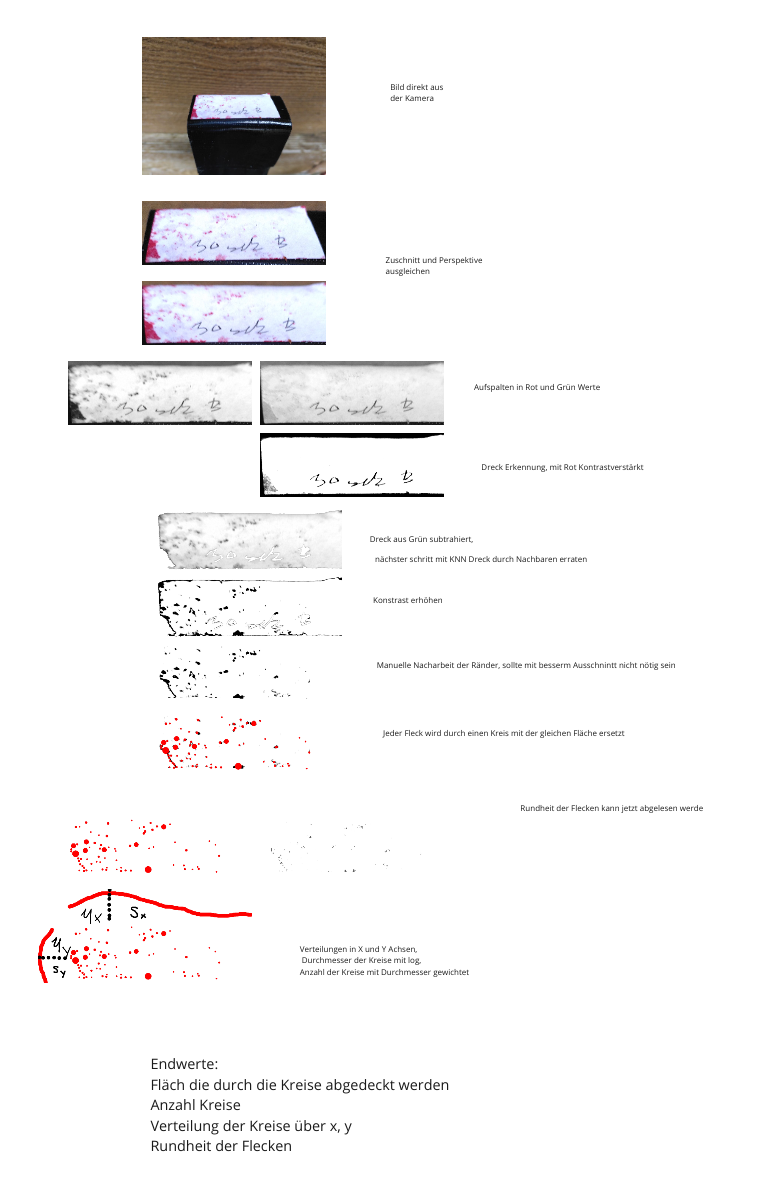
\includegraphics[width=0.9\textwidth]{Bilder/Screenshotfrom2024-04-0112-59-42.png}
    \caption{Bildverarbeitung Konzept}
    \label{fig:Bildverarbeitnugskonzpet}
\end{figure}

\newpage
